\documentclass{article}
\usepackage{graphicx}
\usepackage{amsmath}
\usepackage{natbib}
\usepackage{xcolor}
\usepackage{amssymb}
\newtheorem{proof}{Proof}
\newtheorem{lemma}{Lemma}
\usepackage[margin=1in]{geometry}
\graphicspath{{../figs/}}
\begin{document}


\title{Modifying the Weak Completion Semantics for the Individual Reasoner}
\author{Axel Ind}

\maketitle

\section*{Abstract}
Approaches to cognitive modelling with non-monotonic logics have thus far been largely \textit{ad hoc} and poorly standardised, making inter-model comparisons difficult. As an attempt to systematically represent non-monotonic logics in a framework that standardises cognitive modelling under these logics without sacrificing their expressiveness, we introduce the Sequential Cognition Process (SCP). Under the assumption that human reasoning can be represented as a sequence of distinct cognitive operations on an initial knowledge base SCPs provide a consistent framework for generating and evaluating models of human cognition. Using an adapted interpretation of the Weak Completion Semantics (WCS), SCPs are able to accurately model several classical experiments in cognitive modelling. We use the SCP framework to model both general case reasoners -- which arrive at the most frequently observed conclusions -- and poorly-studied individual case reasoners -- which do not. We illustrate the use of SCPs using the Suppression Task.

\section{Introduction}
The Weak Completion Semantics \citep{holldobler2015weak} is a non-monotonic logical framework which can be used to model the general case of several well-described cognitive tasks. The tasks include but are not limitted to: the Suppression Task \citep{byrne1989suppressing}, the Wason Selection Task \citep{wason1968reasoning}, @TODOmoreTasks. The WCS is one of a number of non-monotonic frameworks \citep{ragni2017formal} which can approximate the empirical results of reasoning tasks.

However, the WCS is primarily concerned with modelling the general reasoner. It has not been tailored to model reasoners whose conclusions differ from the majority response, in this paper we will call these \textit{aberrant reasoners}. Work previously done by \cite{breu2019weak} has shown that, given a suitable sequence of additional steps and constraints to the representation and interpretation of a cognitive task, the WCS can be used to model several of these aberrant cases seen in the Wason Selection Task.

The purpose of this paper is to introduce a well-structured framework for the WCS called a \textit{Sequential Cognitive Process} (SCP) which allows a large number of aberrant cases to be modelled using a limited number of generalised transformations. The benefits of this approach are three-fold: it standardises changes to the WCS which have been largely \textit{ad hoc} to this point; it allows for classical search approaches to explore a well-definited state space of possible models, and thus produce exhaustive sets \footnote{Restricted by the number of allowable operations and their associated sequencing constraints.} of achievable final knowledge states; and enables comparisons between competing congitive models that reach the same conclusions by differing sequences of epistemic operations.

In Section~\ref{sec:prelim} we discuss mathematical preliminaries relating to the Weak Completion Semantics and briefly address concerns regarding the framework used in this paper. Section~\ref{sec:wcs} discusses the formal mathematical features of the WCS framework, and Section~\ref{sec:ecp} introduces several classical experiments which have been well-modelled in this framework. Section~\ref{sec:scp} introduces a sequential framework which encapsulates the WCS and a set of allowable operations that a subject may mentally perform during the completion of a cognitive task. Special attention is paid to the creation of appropriate cognitive operations. The section also demonstrates the ability of the SCP framework to model the previously introduced examples, as well as individual reasoner cases in the same experiments. Section~\ref{sec:comp} introduces the Needleman-Wunsch algorithm and discusses how it can be applied to the SCP framework to deduce the most likely mechanisms by which individual reasoner conclusions are drawn. Section~\ref{sec:conc} ends the paper with a discussion of the framework presented, as well as the strengths and weaknesses its flexibility brings.


\section{Mathematical Preliminaries} \label{sec:prelim}

\subsection{Why Not State Machines}
An obvious question arises after one begins using the definined framework: wouldn't this all be more suitable for a state machine paradigm rather than a planning one? The truth is that both representation structures offer different advantages and disadvantages for the work described in this paper. State diagrams are intuitive, efficient, and well-described in the literature. However, they generally allow more recursive behaviour (i.e. infinite looping) than this paper, which attempts to model the finitely complex thought processes of humans, believes is reasonable. 



@TODOextend. 

\section{The Weak Completion Semantics} \label{sec:wcs}
\subsection{Non-monotonic Logics in General}

Before discussing the WCS, it is important to understand why non-monotonic logics are required for cognitive modelling at all. There are a number of empirical studies demonstrating that humans consistently fail to draw the classically valid conclusions to certain cognitive tasks \citep{byrne1989suppressing}, \citep{wason1968reasoning}. Section~\ref{sec:ecp} describes the Suppression Task, in which human test subjects repeatedly make the mistake of assuming that, given some knowledge base $KB$, it is possible for $KB \models \phi$ to be true, but $(KB \cup \psi) \models \phi$ to be false.

A large number of non-monotonic frameworks exist in the literature \citep{mcdermott1980non}, each applicable to a different subset of cognitive problem space, and each modelling their problem space with various degrees of success. In the simplest formulation, a non-monotonic logic is simply an extension to a classical logic which introduces a preference relation $\rightarrow_p$. This preference relation states that, given some number of derivable facts in a knowledge base, the fact derived using the most preferential rule is to be derived first and cannot be overwritten by a less preferable assignment.

\subsection{The Weak Completion Semantics}

\begin{table}
\begin{center}


\begin{tabular}{ c | c c c }
  $\rightarrow$& $\top$ & $u$ & $\bot$ \\ \hline
 $\top$ & $\top$ & $u$ & $\bot$ \\  
 $u$ & $\top$ & $\top$ & $u$\\  
 $\bot$ & $\top$ & $\top$ & $\top$
\end{tabular}
\caption{A table showing the implication operator in 3-valued \L ukasiewicz logic.}
\label{tbl:luk}

\end{center}
\end{table}

The Weak Completion Semantics is a non-monotonic logic which procedurally encodes several well-known cognitive phenomenon. The WCS makes use of 3-valued \L ukasiewicz logic (Table~\ref{tbl:luk}). It adds abnormalities to non-ground inferences, and replaces the classical inference ($\leftarrow$), with a bijective ($\leftrightarrow$). 

The Weak Completion of a program $P$ is defined as follows:

\begin{enumerate}
\item Replace all clauses of the form $A \leftarrow body_1$, ..., $A \leftarrow body_n$ with $A \leftarrow body_1 \lor ... \lor body_n$.
% \item For all undefined variables $x$, add $x \leftarrow \bot$. THIS IS FOR STRONG COMPLETION ONLY
\item Replace all occurrences of $\leftarrow$ with $\leftrightarrow$.
\end{enumerate}

Applying this procedure to $P$ results in $wcP$ which is the weak completion of $P$.

The next requirement to apply the WCS framework is the introduction of a semantic operator $\phi_{SvL}$ \citep{stenning2008interpretation}. Let $J$ be the result of applying the semantics operator to an interpretation $I$ and logic program $P$. The $J$ is defined as follows:

\[
\begin{split}
J^\top = \{ & A | \textrm{ there exists a clause } A\leftarrow Body \in P \textrm{ with } I(Body) = \top\}
\end{split}
\]
\[
\begin{split}
J^\bot = \{ &  A | \textrm{ there exists a clause } A \leftarrow Body \in P \\
           & \textrm{ and for all clauses } A \leftarrow Body \in P \textrm{ we find } I(Body) = \bot\}
\end{split}
\]

Using $I=<\emptyset, \emptyset>$, the least model ($\textrm{lm}_\textrm{\L}$wc$P$) can be calculated by iterating $\phi_{SvL,P}$.

@TODOextend



\section{Classical Experiments in the WCS} \label{sec:ecp}
The Weak Completion Semantics has found application across a wide range of cognitive modelling phenomena \citep{ragni2017formal}. In this section we limit ourselves to the Suppression Task; the abstract, general, and Deontic cases of the Wason Selection Task; and the @TODO. For each of these tasks, it is important to observe that the WCS is well-suited to modelling the general case, i.e. the most \textit{experimentally common result}. It does not provide any statistical likelihood information, nor explore the space of other possible participant responses.

\subsection{The Suppression Task} \label{ssec:suptask}
The Supression Task is one of the most well-studied cognitive modelling tasks in the literature TODORef. Introduced by \cite{byrne1989suppressing}, it is a clear illustration of the inadequacy of classical logic in modelling human reasoning. One common formulation of the task is the following set of statements:

\begin{itemize}
\item $a$: If Alice has an essay to write ($e$) she will study late in the library ($l$).
\item $b$: If the library is open ($o$), she will study late in the library ($l$).
\item $c$: She has an essay to write ($e$).
\end{itemize}

Told $a$ and $c$, subjects classically conclude that Alice will study late in the library as if applying \textit{modus ponens} ($ \frac{l \leftarrow e, e \leftarrow \top}{l \leftarrow \top}$). However, told $a$, $b$, and $c$, subjects no longer draw this inference, even though it remains classically valid. The additional information affecting the library has somehow \textit{suppressed} the classical inference.

Though the precise reason and mechanism for this phenomenon is still debated, it has been shown that the WCS can be used to mimic the suppressing effect of the additional information.

For the $ac$ case: assume that the initial logic program $P_1$ contains the following facts: $P_1=\{l\leftarrow e \land \lnot ab_1 , e \leftarrow\top, ab_1\leftarrow \bot\}$. As is common in cognitive literature, we introduce the possibility that some abnormal event ($ab_1$) may occur to mean that she does not go to the library, despite having an essay to write. This reason could be anything from illness to, to alien invasions. What is important to note is that we have no additional variables describing these situations, and so the abnormality is assumed to be false. Following the procedure outlined for the WCS, wc$P_1 = \{l\leftrightarrow e \land \lnot ab_1, e \leftrightarrow\top, ab_1\leftrightarrow \bot\}$ and the result of each iteration of the semantic operator is shown in Table~\ref{tbl:suppAC}. In this formulation the variable $l$ is no longer unknown, and so we have concluded in line with classical logic that she will study late in the library.

For the $abc$ case: assume that the initial logic program $P_2$ contains the following facts: $P_2=\{l\leftarrow e \land \lnot ab_1, l  \leftarrow o \land \lnot ab_2, e \leftarrow \top, ab_1\leftarrow \lnot o, ab_2 \leftarrow \lnot e\}$. We follow the same procedure for introducing abnormalities as before, introducing a new abnormality $ab_2$. What is important to understand is that we might consider that along with alien attacks, the library not being open may be a reason Alice would not go to the library, even when she has an essay to write. And, unlike aliens, or unexpected traffic jams, we do have a variable describing if the library is open. Thus, we explicitly state that the library being closed could be the cause of not going there, even when Alice has an essay to write. The same logic holds for the new abnormality $ab_2$, why would she go to the library without an essay to write? Using this new formulation $wcP_2=\{l\leftrightarrow (o \land \lnot ab_2) \lor (e \land \lnot ab_1) , e \leftrightarrow \top, ab_1\leftrightarrow \lnot o, ab_2 \leftrightarrow \lnot e\}$. Now, repeatedly applying the semantic operator gives the results in Table~\ref{tbl:suppABC}. Because no information about $l$ is given in the least model, no conclusion about if Alice will study late in the library can be made.

\begin{table}
\begin{center}

\begin{tabular}{ c c c }
 \textbf{Iteration} & \textbf{$\top$} & \textbf{$\bot$} \\ 
 0 &  &  \\  
 1 & $e$ & $\lnot ab$ \\  
 2 & $e,l$ & $\lnot ab$ \\  
 3 & $e,l$ & $\lnot ab$ 
\end{tabular}
\caption{Applying the Weak Completion Semantics to the $ac$ case of the Suppression Task.}
\label{tbl:suppAC}

\end{center}
\end{table}

\begin{table}

\begin{center}
\begin{tabular}{ c c c }
 \textbf{Iteration} & \textbf{$\top$} & \textbf{$\bot$} \\ 
 0 &  &  \\  
 1 & $e$ &  \\  
 2 & $e$ &  
\end{tabular}
\caption{Applying the Weak Completion Semantics to the $abc$ case of the Suppression Task.}
\label{tbl:suppABC}

\end{center}
\end{table}


\subsection{The Wason Selection Task} \label{ssec:wst}

\begin{table}
\begin{center}


\begin{tabular}{ c c c c c}
  & \textbf{$p$} & \textbf{$pq$} & \textbf{$pq\bar{q}$} & \textbf{$p\bar{q}$}\\ 
 Abstract & 36 & 39 & 5 & 19\\  
 Everyday & 23 & 37 & 11 & 29\\  
 Deontic & 13 & 19 & 4 & 64
\end{tabular}
\caption{The canonical results of the Wason Selection Task}
\label{tbl:can}
\end{center}
\end{table}


Another widely studied task in the psychological literature is the Wason Selection Task (WST), which asks participants to draw conclusions about which variables are able to falsify a given rule (\textit{Modus Tolens}\footnote{If $a\rightarrow b$, then $\lnot b \rightarrow \lnot a$}). We will look at this task in terms of the Abstract case of the task \citep{wason1968reasoning}. Each case is identical to each other in terms of classical logic representation, but each is interpreted differently by subjects. The WST is often used to illustrate that humans do no follow classical logic.

\subsubsection*{Abstract Case}

\begin{figure}
\begin{center}
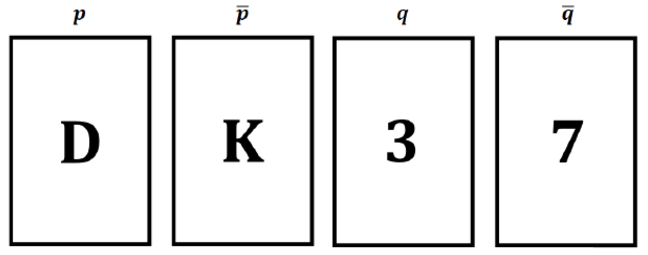
\includegraphics[scale=0.5]{wasonAbstract}
\caption{The Abstract case of the Wason Selection Task}
\end{center}
\end{figure}

The Abstract case of the WST presents the subject with four cards on a table. Their face-up sides read $D, K, 3,$ and $7$. They are asked which cards must be turned over to test the rule:

\begin{center}
``If there is a $D$ on one side of the card, then the other side shows $3$."
\end{center} 
Using classical logic, it is easy to see that turning $D$ to find anything but $3$ would invalidate the rule, as would turning $7$ and finding a $D$. Thus these two cards must be turned to check the rule. However, human subjects very seldom choose this classical answer set and instead overwhelmingly prefer to turn $D$ and $3$. Table~\ref{tbl:can} shows the most common card selection sets for participants.

A great many cognitive theories have been applied to these results, with varying degrees of success \cite{ragni2017formal}. This paper will focus on the WCS interpretation of the task provided by \citep{ragni2017wason}. This approach assumed an initial knowledge base containing only the rule $3 \leftarrow D$.

To illustrate this interpretation of the task we shall use the WCS to examine each of the four cards individually and see what conclusions can be drawn.

When $D$ is observed:

\[
KB = \{3 \leftarrow D, D\leftarrow \top \}
\]

However, at this point, the authors introduce the concept of an abnormality as discussed in \citep{ragni2017formal}. Now, the rule holds only provided that some abnormal even does not occur.

\[
KB_D = \{3 \leftarrow D \land \lnot ab_1, D \leftarrow \top, ab \leftarrow \bot \}
\]

\[
wcKB_D = \{3 \leftrightarrow D \land \lnot ab_1, D \leftrightarrow \top, ab \leftrightarrow \bot \}
\]

The authors also require that, to validate the rule, it must be evaluated after the semantic operator is iterated. Table~\ref{tbl:dcard} shows the result of repeatedly applying the semantic operator to $KB_D$. 

\begin{table}
\begin{center}

\begin{tabular}{ c c c }
 \textbf{Iteration} & \textbf{$\top$} & \textbf{$\bot$} \\ 
 0 &  &  \\  
 1 &  $D$ & $ab$  \\  
 2 &  $D$, $3$ & $ab$  
\end{tabular}
\caption{Applying the Weak Completion Semantics to the $D$ card of the WST.}
\label{tbl:dcard}

\end{center}
\end{table}

When the $K$ card is observed:

\[
KB_K = \{3 \leftarrow D \land \lnot ab_1, K \leftarrow \top, ab \leftarrow \bot \}
\]

\[
wcKB_K = \{3 \leftrightarrow D \land \lnot ab_1, K \leftrightarrow \top, ab \leftrightarrow \bot \}
\]

Table~\ref{tbl:kcard} shows that not enough information can be obtained using only the semantic operator to evaluate the rule $D \leftrightarrow 3$. This is identical to the case for the $7$ card.

\begin{table}
\begin{center}

\begin{tabular}{ c c c }
 \textbf{Iteration} & \textbf{$\top$} & \textbf{$\bot$} \\ 
 0 &  &  \\  
 1 &  $K$ & $ab$  \\  
 2 &  $K$ & $ab$  
\end{tabular}
\caption{Applying the Weak Completion Semantics to the $K$ card of the WST.}
\label{tbl:kcard}

\end{center}
\end{table}

When the $3$ card is observed:
\[
KB_3 = \{3 \leftarrow D \land \lnot ab_1, 3 \leftarrow \top, ab \leftarrow \bot \}
\]

\[
wcKB_3 = \{3 \leftrightarrow D \land \lnot ab_1, 3 \leftrightarrow \top, ab \leftrightarrow \bot \}
\]

In this case, something odd happens. Even though the WCS framework a outlined is not able to deduce anything about the truth value of the variable $D$, participants still very often chose to turn this card. In \cite{breu2019weak} we argue that this may be a result of implicit \textit{abduction}. That is, that the participant subconsciously attempts to identify any possible way in which $3 \leftrightarrow D \land \lnot ab$ could hold when $3=\top$ and $ab=\bot$. The only way for this rule to hold would be for $D$ to be true too:

\begin{table}
\begin{center}

\begin{tabular}{ c c c }
 \textbf{Iteration} & \textbf{$\top$} & \textbf{$\bot$} \\ 
 0 &  &  \\  
 1 &  $3$ & $ab$  \\  
 2 &  $3$ & $ab$  
\end{tabular}
\caption{Applying the Weak Completion Semantics to the $K$ card of the WST.}
\label{tbl:3card}

\end{center}
\end{table}

Now, using Table~\ref{tbl:3card} one can see that $3$ is set to true, the abnormality is set to false, and $D$ has been assumed via abduction. Following \L ukasiewicz logic these assignments are sufficient to evaluate $3\leftarrow D \land \lnot ab$ to $\top$. This the subject will conclude to turn the card.

This simple interpretation of the WST using the WCS and using or not using abduction is sufficient to achieve the most common (general) reasoning of participants. It does not however explain any of the other deviant cases which are observed in Table~\ref{tbl:can}. Why, for example, should it be considered accurate if it gives no information about the classically accurate choice of the $D$ and $7$ cards, chosen by 19 participants, a significant portion? Instead, consider how these aberrant reasoners could be modelled. Perhaps they use extra computational steps or omit steps? This author has previously shown that the WCS is able to model these individual reasoners \citep{breu2019weak} by including two simple processes: Abduction and Contraposition. By including these two processes, and stochastically controlling when they are activated or silenced, it has been shown that not only is this extended framework able to model the major cases of the WCS, but very close approximations to empirical results can also be drawn.

As discussed above, Abduction can be used when the rule under consideration evaluates to unknown. It uses fixing of remaining free varibles to determine if any combination of these can validate or falsify the rule. In the case we have discussed, only fixing $D = \top$ will validate the rule.

Contraposition explicitly makes use of \textit{modus tolens}, usually assumed to be silenced in human cognition to derive certain canonical cases in the WST. In particular, for the card $7$, the logic program:

\[
KB_7 = \{3 \leftarrow D, 7 \leftarrow \top \}
\]

is extended with the rule $\lnot D \leftarrow \lnot 3$, which itself simply means $K \leftarrow 7$ for our restricted domain. 

\[
KB_7 = \{3 \leftarrow D, \lnot D \leftarrow \lnot 3, 7 \leftarrow \top \}
\]

Adding abnormalities yields:

\[
KB_7 = \{3 \leftarrow D \land \lnot ab_1, \lnot D \leftarrow \lnot 3 \land \lnot ab_2, 7 \leftarrow \top, ab_1 \leftarrow \bot, ab_2 \leftarrow \bot \}
\]

After weakly completing:

\[
KB_7 = \{3 \leftrightarrow D \land \lnot ab_1, \lnot D \leftrightarrow \lnot 3 \land \lnot ab_2, 7 \leftrightarrow \top, ab_1 \leftrightarrow \bot, ab_2 \leftrightarrow \bot \}
\]

Applying the semantic operator then yields:

\begin{table}
\begin{center}

\begin{tabular}{ c c c }
 \textbf{Iteration} & \textbf{$\top$} & \textbf{$\bot$} \\ 
 0 &  &  \\  
 1 &  $7$ & $ab_1$, $ab_2$  \\  
 2 &  $K$, $7$ & $D$, $3$, $ab_1$, $ab_2$  
\end{tabular}
\caption{Applying the Weak Completion Semantics and Contraposition to the $7$ card of the WST.}
\label{tbl:7cont}

\end{center}
\end{table}

\begin{figure}
\centering \includegraphics[scale=.6]{wstcano}
\caption{Using the abduction and contraposition extensions to derive all four canonical cases.}
\label{fig:wstcano}
\end{figure}



Table~\ref{tbl:7cont} shows the result of applying the semantic operator to the resulting knowledge base. From this, it is possible to deduce that the card $7$ must be turned. Figure~\ref{fig:wstcano} illustrates the use of these extensions to derive all four of the canonical cases of the WST.

@TODOrewritewholesectionintermsofpq

\section{Extending the WCS Framework} \label{sec:scp}

\subsection{Sequential Cognition Processes}
At this point it is important to restate the intention of this paper: ``to model \textit{non-general} cases of tasks whose general cases are well-characterised by the Weak Completion Semantics." As the intention is to model deviations from normal reasoning, it seems appropriate to attempt to see if small changes to the sequence of thought operations performed might result in the unusual observed cases.

Intuitively, we will treat the thought operations needed to describe human reasoning on a problem as a sequence of well-described operations each of which changes the epistemic state of the individual doing the reasoning. At the end of this sequence, we should observe a belief state that matches the observed empirical results. Such a sequence will be referred to as a \textit{Sequential Cognition Process} (SCP).

\begin{figure}
\centering 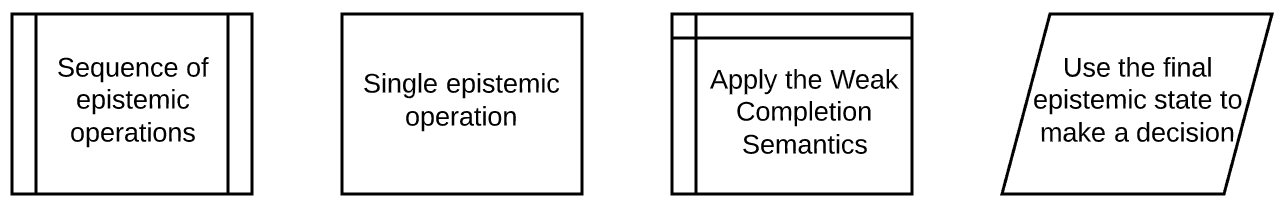
\includegraphics[scale=.6]{allBoxes}
\caption{Simple operations used to describe the WCS framework as a sequence of epistemic operations.}
\label{fig:boxes}
\end{figure}

\begin{figure}
\centering 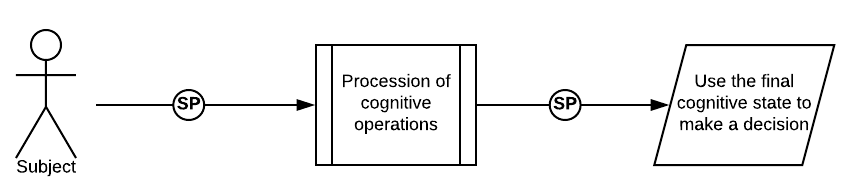
\includegraphics[scale=.36]{general}
\caption{The most simple description of a thought process using epistemic operations.}
\label{fig:general}
\end{figure}

\begin{figure}
\centering \includegraphics[scale=.65]{generalwcs}
\caption{The most simple description of a thought process using epistemic operations in which the WCS is thought to be performed.}
\label{fig:generalWCS}
\end{figure}


To properly illustrate this concept, it is necessary to introduce some diagram notation as seen in Figure~\ref{fig:boxes}. Using this notation, the most generalised case of cognition is shown in Figure~\ref{fig:general}. The origin of solid line arrows indicates indicate an epistemic state resulting from the previous thought operation. The end-point of a solid arrow indicates that a belief state is being used as a knowledge base on which to perform the actions that thought operation requires. Dotted arrows have the same restrictions, exept that exactly one dotted arrow originating from any epistemic operation may be used to reach the desired output. Dotted arrows provide non-deterministic interpretations of SCPs diagrams.

Further restrictions are possible if we wish to model deviations from a task for which the WCS is believed to an adequate model. In this case, it can be assumed that the WCS operation occurs at some point in the SCP\footnote{Later, it will be shown that it is still possible to model deviant users who do not use the WCS by silencing the epistemic operation entirely.} (Figure~\ref{fig:generalWCS}).

For the purposes of this paper, the following limits are placed on the structure of SCPs: because cognitive processing power is finite, yet satisfies a known final $\gamma$ condition, it is reasonable to disallow infinite loops in the SCP; linear SCPs are assumed for computational simplicity; @TODOExtend.

Now it is possible to use SCPs to model general cases of many problems that have been described with the WCS.

\subsection{SCP Formalisation}

An SCP Problem $\Pi = (s_i, \gamma, M, V)$ is a 4-tuple consisting of an an initial state $s_i$, a goal condition $\gamma$, a set of complex operations $M$, and a set of variables $V$. An SCP Problem provides information about epistemic state of a subject as a cognitive task begins, and also describes some condition that must be satisfied when the task is complete.

The initial state $s_i$ is a set of the epistemic ground knowledge of the agent (e.g. $waterIsWet \leftarrow \top$), task-specific information provided by the experiment (``She has an essay to write", $(e \leftarrow \top) \in s_i$), and interpretations of contextual or explicit rules (given ``if she has an essay to write ($e$) she will study late in the library ($l$)'', we might assume $(l\leftarrow e) \in s_i$). Though intuitively simple, this approach also differs significantly from traditional planning because it treats rules as a part of the knowledge base of the system.

The goal state $\gamma$ represents the experimental conclusions that participants in the task had previously drawn. The purpose of SCPs is to begin with a known initial world state and real-world data on general or individualised conclusions, and to draw inferences about the mental operations which caused the derivation of epistemic information in the conclusion. In the case of the Suppression Task, the general reasoner would have no epistemic information about if she will study late in the library $\gamma \models \lnot l \land \lnot (\lnot l)$.

The set of complex operations $M$ is a semi-unconstrained set of ways to manipulate the current epistemic state to reach another, logically valid one. These complex operations correspond to the Epistemic Operations described in Section~\ref{sec:scp}. Structurally, each complex operation $o=<\chi, e>$ consists of a precondition $\chi$ which must hold for the operations to be valid at a given point in the SCP, and an effect $e$ which describes precisely how the epistemic state of the agent will be changed after the operation is completed. Performing the WCS on a knowledge base would consitute a complex action, but so would performing any single part of the WCS (weakly completing, removing duplicate heads in the KB, etc.). It is difficult to provide a mathematically sound definition of complex operations at this level of complexity, but examples provided in Section~\ref{sec:ecp} should illustrate their structure and use.

Finally, the set of variables $V$ describes those variables which appear in the SCP and their assignments. Unlike in traditional planning, some $v \in V$ at the time of operation $o_n$ was not necessarily in $V$ at the time of operation $o_{n-1}$ and their is no requirement that is remains after $o_{n+1}$. This ability to add and remove variables from the epistemic state will be shown to be very helpful in modelling certain tasks using SCPs.

Now, armed with the tools to understand an SCP Problem, we can define an SCP itself. An SCP ($\pi=s_i o_1 o_2 ... o_n)$ describes a sequence of valid complex operations which transform the initial epistemic state to some final epistemic state $s_n$. State $s_i$ is definied by $s_i = s_{i-1} o_{i}$. If $s_n \models \gamma$ and every complex operation $o_i$ is applicable in state $s_{i-1}$, $\pi$ is said to be a valid SCP.

\subsection{Selecting Complex Operations}

It is apparent that this approach requires a robust set of usable operations in order to model human reasoning. For example, if our final mental state $s_n \models \phi \leftarrow \top$, then either $\phi$ must be set to $\top$ in the initial epistemic state, or there must be some operator that has an effect which leaves $\phi$ set to $\top$. Further, there should be some valid sequence of complex operators which can transform the initial epistemic state of the agent to some in which $\phi$ holds. If no such sequence exists, then the SCP is trivially inadequate to model the experimental results being considered. Thus, a significant portion of the work of creating SCPs relates to specifying a powerful, well-defined, and cognitively reasonable set of complex operations that are applicable across several sets of experimental data.

Though this is a daunting task, there are some absolute requirements for the set of complex operators $M$ in an SCP:

\begin{enumerate}
\item Some $M' \subseteq M$ must be powerful enough to apply the weak completion semantics to some state $s_n$\footnote{This paper concerns itself with modelling both the general and individual cases of cognitive experiments with the WST, so the WST must be possible in this framework.}.
\item Some $N' \subseteq M$ must be powerful enough to create abnormality variables in rules. It must also be powerful enough to create auxiliary rules assigning truth values to those abnormalities.
\end{enumerate}

Further, some commonsense requirements present themselves\footnote{In time it may be shown that some of these operators are not cognitively valid, but they present an effective and intuitive starting point.}:

\begin{enumerate}
\item It should be possible to create new epistemic variables.
\item It should be possible to remove existing epistemic variables, at least in trivial cases.
\item It should be possible to silence other epistemic operations.
\item For reasons related to the Needleman-Wunsch algorithm (Section~\ref{sec:comp}) it should not be possible to rearrange complex operators in the SCP\footnote{The same effect can be achieved by a series of silencing and new operators.}.
\end{enumerate}

Finally, $M$ should contain epistemic operations whose existence is well-substantiated by the psychological literature:

\begin{enumerate}
\item Variable fixing: it follows from work such as the excellent \cite{griffiths1994role} that participants in psychological experiments sometimes hold over biases in their cognitive reasoning. That is, they may often be unwilling to change their epistemic state about a variable, even when presented with direct evidence that they are incorrect. This is a problem that is often encountered in the real world. For example in jury biases often lead to immutable conclusions about aspects of a case, even when evidence directly contradicts their beliefs \citep{bray1978authoritarianism}	.
\item @TODOfindABunchOfLikelyPhenomena
\end{enumerate}

\begin{figure}
 \centering 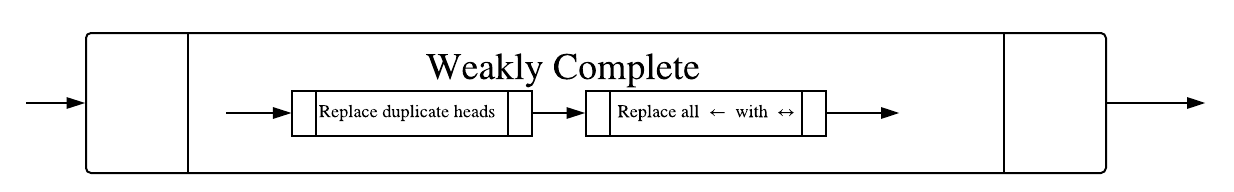
\includegraphics[scale=0.75]{weaklycompleteSCP}
\caption{An SCP segment showing the two steps in the WCS.}
\label {fig:broadWCS}
\end{figure}

\begin{figure}
 \centering 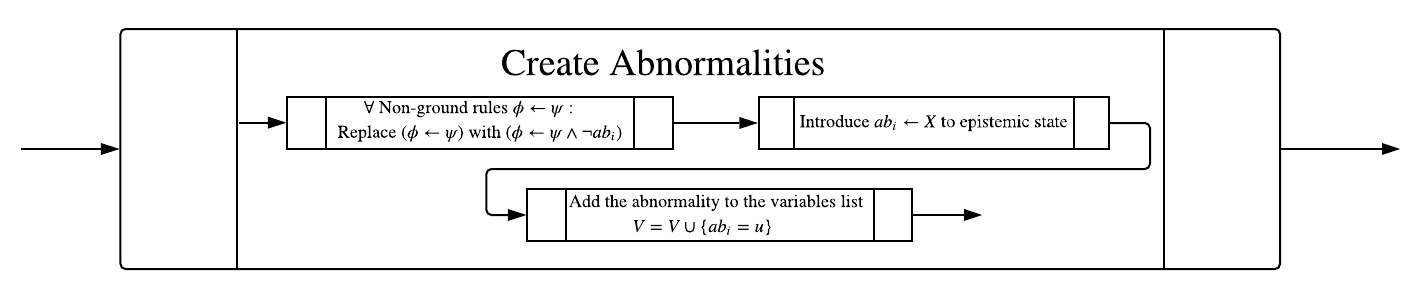
\includegraphics[scale=0.75]{abnormalitySCP}
\caption{An SCP segment showing the three steps in the creation of abnormality variables in an SCP. Where $X = x_1 \land ... \land x_n$, for all $x_i \models \phi$. That is, $x_i$ is a variable that would be considered an abnormal event.}
\label {fig:abnormality}
\end{figure}

\begin{figure}
 \centering 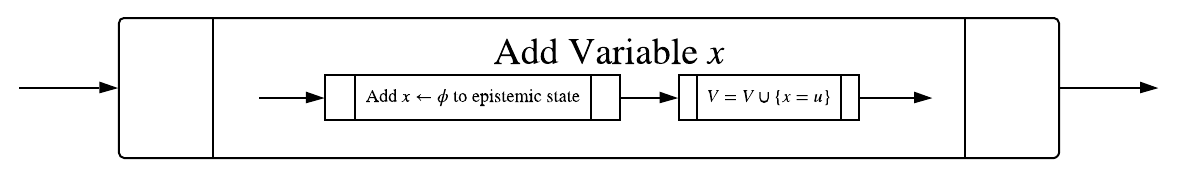
\includegraphics[scale=0.75]{addVariableSCP}
\caption{An SCP segment showing the steps in the addition of a new variable to the cognitive state.}
\label {fig:addVariable}
\end{figure}

\begin{figure}
 \centering 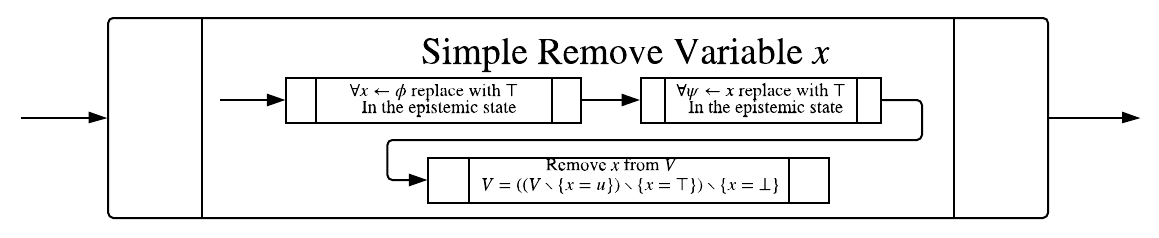
\includegraphics[scale=0.75]{removeVariableSCP}
\caption{An SCP segment showing the steps in the removal of an existing variable to the cognitive state. The variable is assumed to exist only in the head of clauses in the epistemic state. More complex removals require a case-by-case examination.}
\label {fig:removeVariable}
\end{figure}

\begin{figure}
 \centering 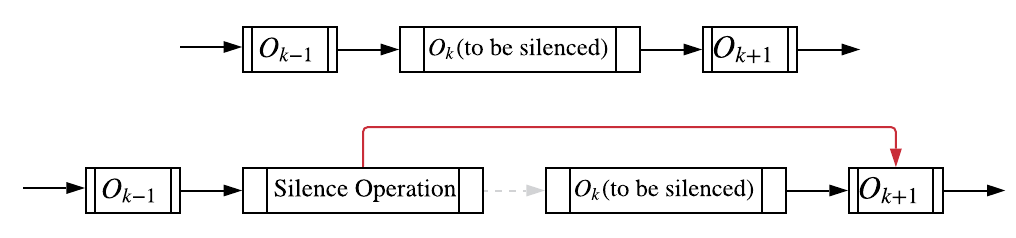
\includegraphics[scale=0.75]{silenceSCP}
\caption{An illustration of the effect of the silencing operation in an SCP. It causes the effect of the next complex action taken to be the empty set and moves on to the next cognitive operation.}
\label {fig:silence}
\end{figure}

\begin{figure}
 \centering 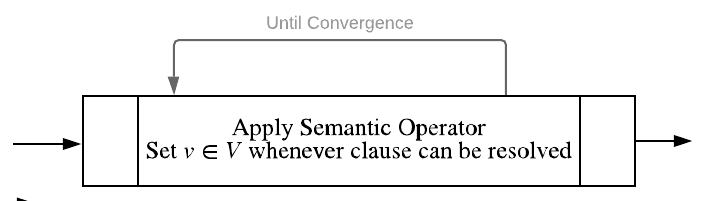
\includegraphics[scale=0.75]{semanticOperatorSCP}
\caption{An illustration of the effect of the semantic operator in an SCP environment. Though it contains a loop, the use of \L ukasiewicz logic guarantees convergence to a least model. }
\label {fig:semantic}
\end{figure}



Figure~\ref{fig:generalWCS} illustrates one possible representation of the weak completion process as an SCP. The two sub-processes shown within are those already discussed in Section~\ref{sec:scp}. It is important to note that any internal representation of the weak completion operation could be used, provided that the epistemic state achieved at the end is consistent with our definition of weak completion. Because their is no precondition for weakly completing an epistemic state, the $<\chi, e>$ format is simplified only to show the effect $e$ of the process, this convention will be followed throughout this paper.

Other possible representations for complex actions discussed are Figure~\ref{fig:abnormality} for introducing abnormalities, Figure~\ref{fig:addVariable} for adding new variables, Figure~\ref{fig:removeVariable} shows the removal of a variable, Figure~\ref{fig:semantic} shows the use of the Semantic Operator, and Figure~\ref{fig:silence} shows the effect of the silence operation on an SCP.

It is important to note that the silence operation differs from all other SCP operators because it affects another operator. This unique behaviour is necessary, and the silence operator at SCP position $t$ changes the operator at position $t+1$ ($o_{t+1}$) of the form $<\chi, e>$ and changes it to the form $<\top, \top>$ until SCP position $t+2$ is reached, at which point the operator is reverts to its original form for all subsequent occurrences.



\subsubsection{Suppression Task} \label{ssec:supTaskCPD}

\begin{figure}
\begin{center}
 \centering 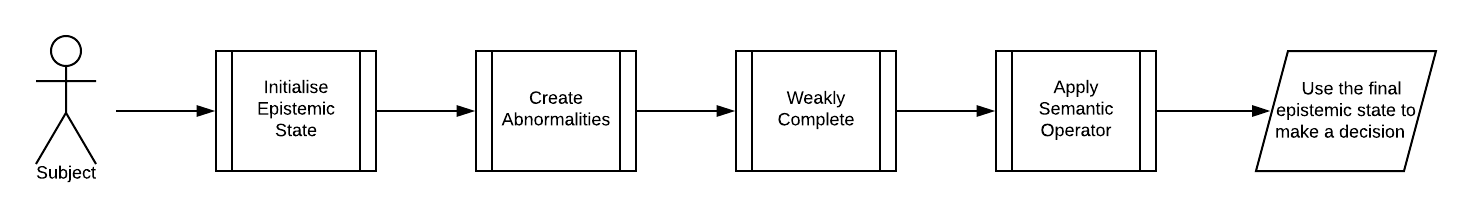
\includegraphics[scale=0.75]{suppressionSCP_overview}
\caption{A generalised illustration of the WCS in an SCP. }
\label {fig:supoverview}
\end{center}
\end{figure}

\begin{figure}
\begin{center}
 \centering 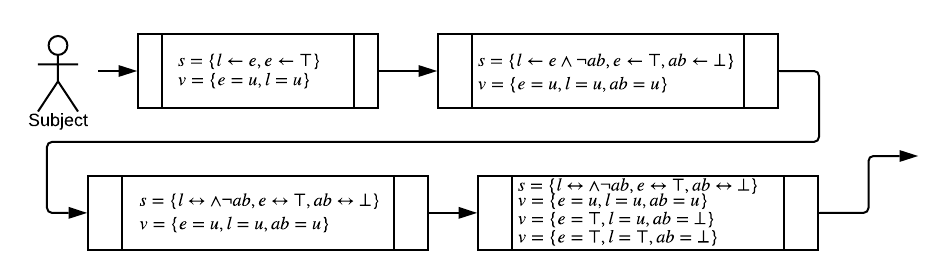
\includegraphics[scale=0.75]{suppressionSCP_simple}
\caption{The first case of the Suppression Task, without the additional conditional. }
\label {fig:supsimple}
\end{center}
\end{figure}

\begin{figure}
\begin{center}
 \centering 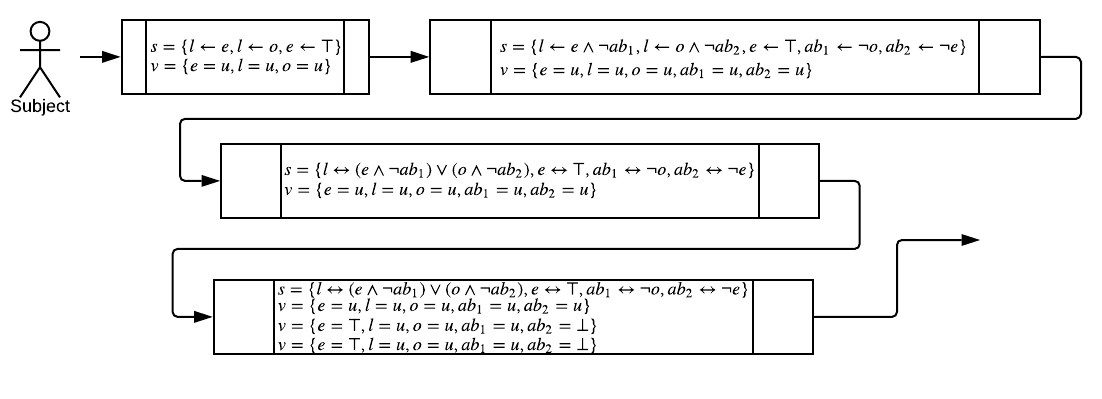
\includegraphics[scale=0.75]{suppressionSCP_normal}
\caption{The standard case of the Suppression Task, demonstrating the suppression effect. }
\label {fig:supnormal}
\end{center}
\end{figure}

\begin{figure}
\begin{center}
 \centering 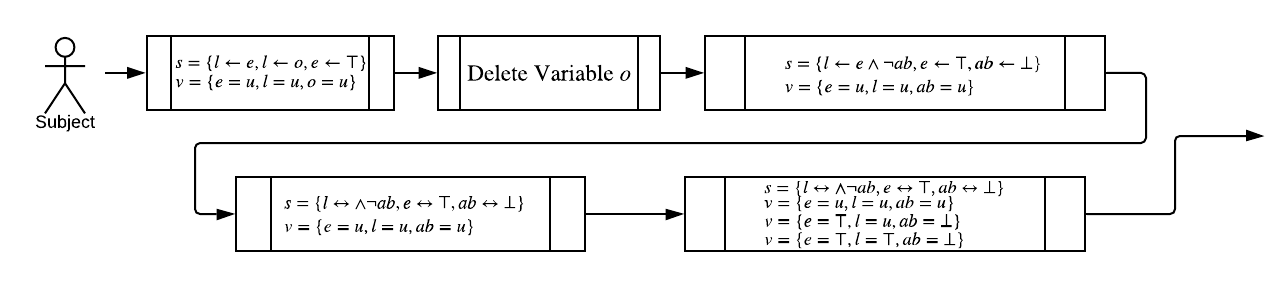
\includegraphics[scale=0.75]{suppressionSCP_mod}
\caption{A modified version of the Suppression Task SCP in which variable $o$ is ignored. }
\label {fig:supmod}
\end{center}
\end{figure}

\begin{figure}
\begin{center}
 \centering 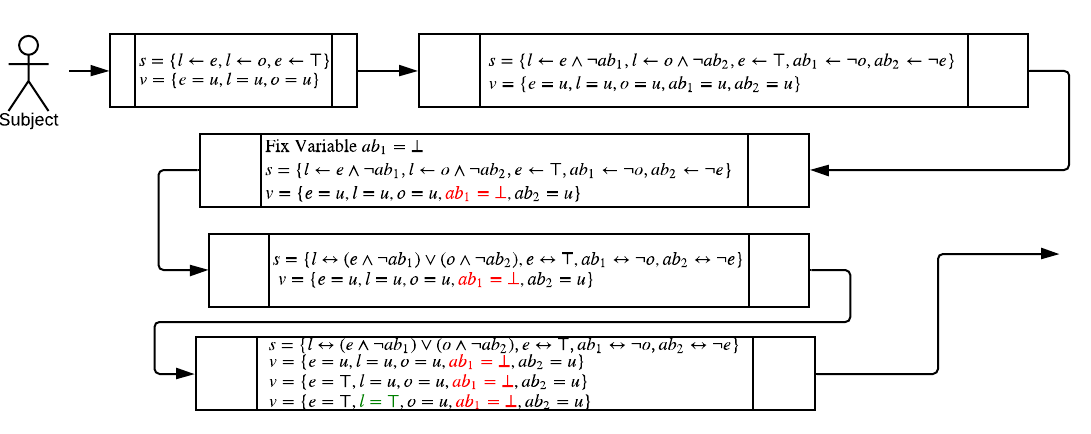
\includegraphics[scale=0.75]{suppressionSCP_mod2}
\caption{A modified version of the Suppression Task SCP in which variable $ab_1$ is fixed to false. }
\label {fig:supmod2}
\end{center}
\end{figure}

In order to mimic the WCS interpretation of the suppression task, several sequential actions are required. First, the initial knowledge base must be generated by the user. For this purpose, appending the facts and rules to the knowledge base is represented using one epistemic operation. After the knowledge base is generated, information about abnormalities is encoded with another epistemic operation. Applying the WCS framework (including semantic operator) to the completed knowledge base results in an epistemic state that still leaves $l$ neither True nor False, and thus, no conclusion is drawn (Figure~\ref{fig:supnormal}).




The general process followed for applying the WCS in an SCP is given in Figure~\ref{fig:supsimple}, and should come as no surprise. It makes use of components introduced in Section~@TODOref and follows an intuitive sequence of steps to achieve the same results as seen in Section~@TODOsec.

Following this outline, one is able to effectively model both the simplified version of the Suppression Task (Figure~\ref{fig:supsimple}) and the full task (Figure~\ref{fig:supnormal}). This serves to demonstrate that SCPs are able to model the general case of the Suppression Task. But now we can address the question of if this framework is able to model non-general reasoners, are we able to mimic other conclusions drawn in experimentation? The answer appears to be that we can.

Figure~\ref{fig:supmod} shows what happens if the additional variable $o$ is ignored. It is important to note that this does not necessarily mean that the test subject has completely forgotten that the variable exists, simply that, for whatever reason, they have not included it in their reasoning about this specific problem. In the case that variable $o$ is forgotten, the reasoning process now closely follows that seen in Figure~\ref{fig:supsimple}, and it is deduced that she will study late in the library. It is important to note that, although this is the classical answer to the problem, it was reached using principles in non-monotonic logic and the additional operator flexibility provided by SCPs.

There exist other ways to achieve this non-general answer using the SCP framework and Section~TODOref will concern itself with a discussion on how to choose the most appropriate sequence of operations, and which sequences are most plausible. Figure~\ref{fig:supmod2} demonstrates another intuitive way in which the classical logic result may be achieved. By fixing the subject's $ab_1$ variable before application of the semantic operator, we are able to force an unexpected result. The intuition behind this approach is that the subject may not believe that anything can derail the intention to study in the library when their is an essay to write, regardless of external factors.

A comparison of these two candidate solutions will be provided later in Section~\ref{sec:comp}.




\subsubsection{Wason Selection Task} \label{ssec:WSTCPD}


\begin{figure}
\begin{center}
 \centering 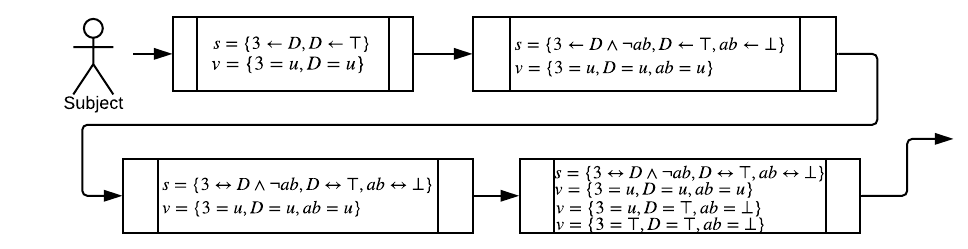
\includegraphics[scale=0.75]{WSTSCPD}
\caption{An SCP representing the WST when the card D is seen. }
\label {fig:wstscpD}
\end{center}
\end{figure}

\begin{figure}
\begin{center}
 \centering 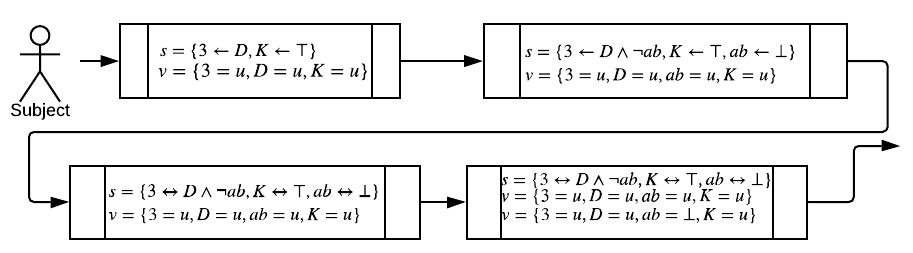
\includegraphics[scale=0.75]{WSTSCPK}
\caption{An SCP representing the WST when the card K is seen. }
\label {fig:wstscpK}
\end{center}
\end{figure}

\begin{figure}
\begin{center}
 \centering 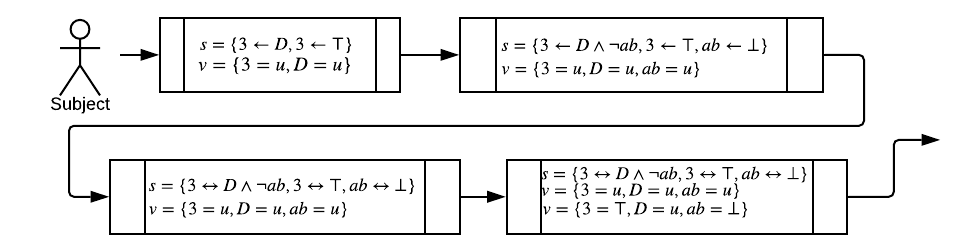
\includegraphics[scale=0.75]{WSTSCP3}
\caption{An SCP representing the WST when the card 3 is seen. }
\label {fig:wstscp3}
\end{center}
\end{figure}

\begin{figure}
\begin{center}
 \centering 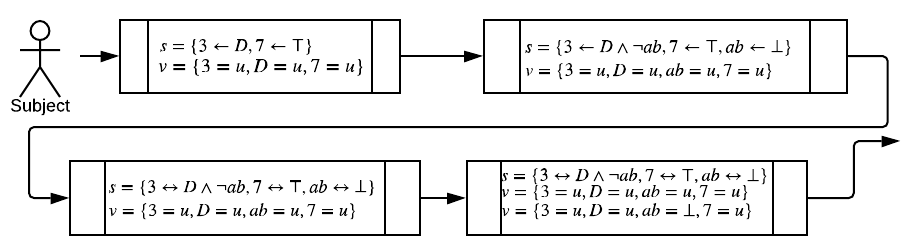
\includegraphics[scale=0.75]{WSTSCP7}
\caption{An SCP representing the WST when the card 7 is seen. }
\label {fig:wstscp7}
\end{center}
\end{figure}



Following the same programmatic intuition we used for the Suppression Task (Figure~\ref{fig:supoverview}), we can create an SCP to model the WST. As in Section~\ref{ssec:wst} it is necessary to create a weakly completed program for each of the four cards. This allows subjects to consider each card in isolation and determine whether it should be turned over\footnote{The adequacy of this isolationist approach is questionable @TODOref, but will be considered sufficient for the purposes of this paper.}. Figures~\ref{fig:wstscpD}, \ref{fig:wstscpK}, \ref{fig:wstscp3}, and \ref{fig:wstscp7} illustrate one possible SCP for the cards $D$, $K$, $3$, and $7$, respectively. This approach is sufficient to represent the most common card selection combination $D,3$, but not any of the other canonical cases seen in Table~\ref{tbl:can}.

@TODOcompleteandredodiagrams


\subsection{Systematically Generating SCPs}

Thus far we have followed an intuitionist approach to modifying General SCPs so that their output matches the observed results of aberrant reasoners. Though this approach can be effective, and mirrors the largely \textit{ad hoc} approach to cognitive modelling that is common in the field, it is not exhaustive or systematic. One of the great advantages of using the SCP framework with a limited set of complex operators is the potential for systematic searching of possible SCPs to find both the initial General SCP that models the general reasoner, as well as extending that SCP to model the aberrant reasoner. The similarity of SCPs transition mechanics to those found in traditional planning mean that a large number of the algorithms that can be used for search in a planning paradigm remain applicable here (albeit now with unbounded time and space complexity).

Consider the Breadth First Search Algorithm (BFS) @TODOinappendix, in which every possible next state reachable from the current state is explored before doing the same for each expanded child node until the desired result is found. It is not hard to formalise this algorithm for SCPs @TODOformalise. Using this approach and the set of complex operations we have already discussed it becomes a simple matter to find possible SCPs that model general case reasoning for the Suppression Task.

\subsection{Heuristics for SCPs}


\subsection*{SCPs for deviant reasoning}


\subsubsection*{Suppression Task}
@TODO

\subsubsection*{Wason Selection Task}
@TODO

\section{Comparing Model Feasibilities} \label{sec:comp}

\subsection{Why Should We Compare Models?}
Thus far, we have been concerned with finding possible ways to modify general WCS models to explicitly describe the reasoning of aberrant reasoners. It is also trivially provable (Proof~\ref{prf:infinitelyLong}) that if there is any SCP that models some cognitive phenomenon, then there are infinitely many possible alternative SCPs which also model that process. In order to compare two SCPs and determine which is more feasible (i.e. a better model of human cognition for this individual reasoner case) we borrow some ideas from the field of bioinformatics.

Scoring SCPs at the time of generation is a fairly simple affair, and it may suffice simply to assign a scoring scheme for each operator that must be added to the general case SCP to model the results of the aberrant reasoner. However, comparing Aberrant SCPs based on different underlying General SCPs is an important but complex task, and requires specialised algorithms to be computationally viable.

Specifially, we will make use of the Needleman-Wunsch Algorithm \citep{needleman1970general}, most often used to compare two DNA sequences to one other. The algorithm is underlied by the principle that two genetic sequences can be related to one another and have simply changed independently over evolutionary time. The purpose of the algorithm is to roughly estimate some kind of similarity by descent between the two sequences. Great emphasis has been put on the sequential requirement for SCPs up to this point, and now the importance of this restriction becomes evident.



 \subsection{The Needleman-Wunsch Similarity Scoring Algorithm}
\begin{table}
\begin{center}

\begin{tabular}{ c | c c c c c}
 D&&A&A&C&G\\ \hline
 & \textcolor{green}{0} & -2 & -4 & -6 &  -8 \\
 A & -2 & \textcolor{green}{1} & -1 & -3 & -5  \\
 A & -4 & -1 & \textcolor{green}{2} & 0 &  -2 \\
 T & -6 & -3 & \textcolor{green}{0} & 1 & -1 \\
 C & -8 & -5 & -2 & \textcolor{green}{1} & 0 \\
 G & -10 & -7 & -4 & -1 & \textcolor{green}{2} 
\end{tabular}
\caption{The Needleman-Wunsch Algorithm for similarity scoring applied to the strings \textit{AACG} and \textit{AATCG}. Entries in green are part of the optimal traceback. Match: 1, Mismatch: -1, Insertion: -2, Deletion: -2}
\label{tbl:need1}

\end{center}
\end{table}

The Needleman-Wusch algorithm is an efficient ($O(n^2)$ time, $O(n^2)$ space) algorithm for comparing two strings. The algorithm determines the minimum number of operations needed to transform one string into the other. The basic principle of the algorithm is to compare the two strings in a matrix. Each cell of the matrix $(row,col)$ represents the minimum number of operations needed to transform the substring [col,0] of the first word into the substring [0,row] of the second word. 

The Needleman-Wunsch algorithm recognises 3 basic operations: match/mismatch, insertion, and deletion. A match/mismatch denotes a case where the two letters are assumed to be in the correct position relative to once another and are either identical (a match), or dissimilar because the letter has been changed (a mismatch). An insertion denotes a case there is assumed to be a letter missing from the first string that existed in the second. Finally, a deletion denotes a case where there is a letter in the first string that is assumed to be absent from the second string. The recursion for the Needleman-Wunsch algorithm is as follows:

\begin{equation}
 D_{ij} = \textrm{max} \left( \begin{matrix} 
      & D_{i-1,j-1} & + &\textrm{match}  \\
     &  D_{i-1,j-1} & + &\textrm{mismatch}  \\
      & D_{i-1,j} & + &\textrm{insertion}   \\
     & D_{i,j-1} & + &\textrm{deletion}   \\
   \end{matrix} \right)
\end{equation}

Entries with higher scores are assumed to be more similar. Table~\ref{tbl:need1} shows the maximum score of the operations needed to turn the string $AACG$ into the string $AATCG$, assuming the given score chart. The entry at the bottom right of the matrix denotes the maximum score for match the entire sequences to once another. Starting from the bottom right and working back along a viable recursion route results in a traceback that can be used to identify the actual sequence of operations need to transform the two strings into one another.

\subsection{Needleman-Wunch and SCPs}

\begin{table}
\begin{center}

\begin{tabular}{ c c }
 \textbf{Process} & \textbf{Score} \\ 
 Match & 1 \\
 Mismatch & -1 \\
 Insert & -2 \\
 Delete & -2
\end{tabular}
\caption{A very simple table for scoring SCPs with the Needleman-Wunsch algorithm.}
\label{tbl:simpleneed}

\end{center}
\end{table}


\begin{table}
\begin{center}

\begin{tabular}{ c | c c c c c c}
& & init & addAB & weakly  & SO & SO \\ \hline
& \textcolor{green}{0} & -2 & -4 & -6 & -8 & -10 \\

init & -2 & \textcolor{green}{1} & -1 & -3 & -5 & -7 \\

delete & -4 & \textcolor{green}{-1} & 0 & -2 & -4 & -6 \\

addAB& -6 & -3 & \textcolor{green}{0} &-1 &  -3 & -5 \\

weakly& -8 & -5 & -2 & \textcolor{green}{1} & -1 & -3 \\

SO & -10 & -7 &  -4 & \textcolor{green}{-1} & 2 & 0 \\

SO & -12 & -9 & -6 & -3 & \textcolor{green}{0} & 3\\

SO & -14 & -11 & -8 & -5 & -2 & \textcolor{green}{1} 
 
\end{tabular}
\caption{The Needleman-Wunsch Algorithm for scoring the similarity of $s_1$ and $s_2$. Entries in green are part of the optimal traceback. Match: 1, Mismatch: -1, Insertion: -2, Deletion: -2}
\label{tbl:needs1s2}

\end{center}
\end{table}

\begin{table}
\begin{center}

\begin{tabular}{ c | c c c c c c}
& & init & addAB & weakly  & SO & SO \\ \hline
& \textcolor{green}{0}  & -2  & -4 & -6  & -8  & -10 \\

init & -2 & \textcolor{green}{1} & -1 & -3 & -5 & -7 \\

addAB & -4 & -1 & \textcolor{green}{2} & 0 & -2 & -4 \\

fix &-6 & -3 & \textcolor{green}{0} & 1 & -1 & -3  \\

weakly& -8& -5 & -2 & \textcolor{green}{1} & 0 & -2  \\

SO & -10& -7 & -4 & \textcolor{green}{-1} & 2 & 1  \\

SO & -12& -9 & -6 & -3 & \textcolor{green}{0} & 3  \\

SO & -14 & -11 & -8 & -5 & -2 & \textcolor{green}{1}  \\
 
\end{tabular}
\caption{The Needleman-Wunsch Algorithm for scoring the similarity of $s_1$ and $s_3$. Entries in green are part of the optimal traceback. Match: 1, Mismatch: -1, Insertion: -2, Deletion: -2}
\label{tbl:needs1s3}

\end{center}
\end{table}

A linear SCP can be represented using a single string. For example the SCP for the Suppression task (Figure~\ref{fig:supnormal}) might be represented with the string:

\[s_1=init-addAB-weaklyComplete-SO-SO\]

Which simply denotes the sequence of complex actions in the SCP. Similarly, our two modified SCPs for the deviant case can be denoted as follows:


\[s_2=init-deleteO-addAB-weaklyComplete-SO-SO-SO\]

\[s_3=init-addAB-FixVariable-weaklyComplete-SO-SO-SO\]

Given these strings, and a suitable scoring matrix, it is possible to use a modified version of the Needleman-Wunsch algorithm to estimate the similarity between the original sequence $s_1$ and our two proposed deviations $s_2$ and $s_3$.

%What is important to note is that, unlike in the Needleman-Wunsch algorithm where every part of the sequence shares a single type (i.e. nucleotide, polypeptide, ...)

Creating a scoring matrix for SCPs becomes a very interesting problem. An extremely simple one might look something like Table~\ref{tbl:simpleneed}. This follows an identical pattern to the original algorithm, and the corresponding scoring matrix is given in Table~\ref{tbl:needs1s2} for $s_1$ and $s_2$, and in Table~\ref{tbl:needs1s3} for $s_1$ and $s_3$. USing the Needleman Wunsch algorithm and looking at the traceback, one can see that both comparisons assign a similarity score of 1, but the traceback itself differs.

However, these tables makes one significantly questionable assumption. In the normal Needleman-Wunsch algorithm every part of the sequence shares a single type (i.e. nucleotide, polypeptide, etc). This is emphatically not the case for SCPs where every part of the sequence represents a complex epistemic process. Some of these processes might be very easily and frequently used in reasoning, whereas other might happen only exceedingly rarely. These complex operations might differ markedly from one another. For this reason, the standard Needleman-Wunsch algorithm is inadequate. What is needed is a modification which allows for each type of epistemic operation to be scored independently. This necessitates a table for each operation that details the score for inserting, deleting, matching, or mismatching that particular operation.


\begin{table}
\begin{center}

\begin{tabular}{ c c c c c c c}
 \textbf{Process} & \textbf{init} & \textbf{addAB} & \textbf{weak} & \textbf{SO} & \textbf{fix} & \textbf{delete}\\ 
 Match & 1 & 1 & 1 & 0 & 1 & 1\\
 Mismatch & -2 & -1 & -1 & 0 & -1 & -3\\
 Insert & -1 & -2 & -2 & 0 & -2 & -3\\
 Delete & -1 & -2 & -2 & 0 & -2 & -3
\end{tabular}
\caption{An arbitrary table for scoring SCPs with the extended Needleman-Wunsch algorithm.}
\label{tbl:arbneed}

\end{center}
\end{table}



\begin{table}
\begin{center}

\begin{tabular}{ c | c c c c}
& & init & addAB & weakly  \\ \hline
& 0 & -1 & -3 & -5  \\

init & -1 & 1 & -1 & -3 \\

delete & -4 &-2  & -2 & -4 \\

addAB & -6 & -4  & -1 & -3 \\

weakly & -8 & -6 & -3 & 0   \\
 
\end{tabular}
\caption{The Needleman-Wunsch Algorithm for scoring the similarity of $s_1$ and $s_2$, using the extended scoring table Entries in green are part of the optimal traceback.}
\label{tbl:exneeds1s2}

\end{center}
\end{table}


\begin{table}
\begin{center}

\begin{tabular}{ c | c c c c}
& & init & addAB & weakly  \\ \hline
& 0 & -1 & -3 & -5  \\

init & -1 & 1  & -1 & -3 \\

addAB & -3 & -1  & 2 & 0 \\

fix & -5 & -3 & 0 & 0 \\

weakly & -7 & -4 & -2 & -1   \\
 
\end{tabular}
\caption{The Needleman-Wunsch Algorithm for scoring the similarity of $s_1$ and $s_3$, using the extended scoring table Entries in green are part of the optimal traceback.}
\label{tbl:exneeds1s3}

\end{center}
\end{table}


At present, no analysis of existing psychological phenomena and congitive process frequencies with regards to SCPs exists. Until one is created, it suffices to use commonsense scoring mechanisms to demonstrate the suitability of the algorithm for SCPs, if not yet its usefulness. We might, for example, assume that variable fixing (as in $s_3$) is much more likely likely than variable deletion (as in $s_2$). Further we might consider that repeated applications of the semantic operator are negligibly informative about the cognitive state of the subject and so the number of times it is applied ignored entirely. An example of an extended scoring matrix that reflects this hypothesis is given in Table~\ref{tbl:arbneed}. 

One convenient advantage of setting our own table values, means that we can omit the semantic operator complex operation from subsequent tables, as we have set all of its values to 0 and it no longer affects the recursion.

Tables~\ref{tbl:exneeds1s2} and \ref{tbl:exneeds1s3} show the results of using the new scoring system on $s_1s_2$ and $s_1s_3$ respectively. Now final scores of the tables do differ. It appears that, under the assumption than deleting a variable is more mentally expensive than fixing one, $s_3$ is the more cognitively consistent approach to explaining the deviation in the Suppression Task where the classically correct answer is derived.

\subsection{Extensions and Notes}

The Needleman-Wunsch algorithm is generally considered a good introductory algorithm to those learning bioinformatics, it lacks many of the useful features of more advanced algorithms in the field. In a similar way, it was used here to show the suitability of similarity scoring algorithms to SCPs, logical extensions to more advanced string-matching algorithms are easily imagined.

A significant limitation of the Needleman-Wunsch algorithm, and by extensions our algorithm, is the inability to deal with crossovers. That is, the algorithm cannot handle cases where operators or groups of operators are shifted into a new position (imagine cutting the middle out of a piece of string and retying it to the end of the string). This limitation is imposed by many such algorithms to limit the computational complexity of the computation, without this limitation string matching becomes NP-hard.

The Smith-Waterman algorithm \citep{smith1981identification} is a simple variation on the Needleman-Wunsch algorithm and is used to  find optimal local alignments. It could be used to find subsequences of complex actions that are preserved between different SCPs. These subsequences (for example $addAB - weaklycomplete$) may be shown to be present in comparisons of models of different cognitive tasks, and may be considered to show support for common motifs in general human cognition.

\section{Conclusion} \label{sec:conc}

This paper has served to introduce SCPs and to show their applicability across a number of cognitive experiments which were well-characterised by the weak completion semantics. Further, it has show the suitability of SCPs for extending general WCS models to describe deviant reasoners. Finally, this paper introduced a variation on the Needleman-Wunsch Algorithm for string matching which was able discern which of several candidate SCPs is most likely to explain deviant experimental results. Under the assumption that non-standard reasoners are deviations from the general reasoners, the Needleman-Wunsch algorithm is a well-founded approach to quantifying SCP similarities. (@TODOdiscussREgularEpressionRepresentationOfSCPs)

\newpage
	
\bibliography{bibl}
\bibliographystyle{chicago}

\newpage
\section*{Appendix}
\begin{proof}
Let $\pi = s_i m_0 ... m_n$ be a valid SCP. If $\pi \models \phi$ then there exist infinitely many other SCPs $\Pi'$ each of which also models $\phi$:

\begin{enumerate}
\item Let $s \in M$ be a silencing operation.
\item  Let $n \in M$ be any arbitrary complex operation
\item Let $\pi'= \pi \cup sn$ @TODOmustdefineoperationsonSCPs
\item $\pi' \models \phi$ (because $s$ silences $n$ and $\pi \models \phi$. 
\item This can be iterated infinitely often using $\pi = \pi'$.
\end{enumerate}

\label{prf:infinitelyLong}
\end{proof}


\begin{lemma}
The number of ways of rearranging a string $s$ of length $l$ into a new string $s'$ s.t. some number $k$ letters of the sequence of retain their ordering (that is: if $q_i \succ q_{j}$ in s, then $q_i \succ q_{j}$ in $s'$) is given by $n_k = \begin{pmatrix}
     l \\ l-k
  \end{pmatrix}$. 
  
  For example, there are 24 ways to rearrange the letters $``abCD"$ if there are no constraints on order $\begin{pmatrix} 4 \\ 4 \end{pmatrix}$, but only one way  $\begin{pmatrix} 4 \\ 0 \end{pmatrix}$ to rearrange the same string if we impose the restriction ($a \succ b \succ C \succ D$).
\label{lem:rear}
\end{lemma}
\begin{proof}
The number of ways of inserting a string $M'$ of length $k$ into a string $s$ of length $l$ to create a new string $S$ under the constraints:
\begin{enumerate}
\item Every $m \in M'$ appears in $S$ \textbf{once and only once}.\footnote{Even if the same action appears multiple times in $M'$ each is treated as a unique and separate action from the others.}
\item Every letter $p\in s$ appears in $S$ once and only once.
\item The order of letters in $s$ is preserved in $S$ for all letters in $s$. That is, if $\forall x, y \in s$, if $x \succ y$ in $s$, then $x \succ y$ in $S$.
\item $\nexists p \in S$ s.t. $p \not\in s$ and $p \not\in M'$. For a single letter $p$.

is given by the equation:

\[
n_k =\begin{pmatrix} l + k \\ k \end{pmatrix}.
\]

\end{enumerate}

\begin{itemize}
\item Introduce string $s'=s+M'$. $s'$ has length $l+k$. 
\item By enforcing the order requirement of $s$ (@TODOref) on $s'$ we specify a string in which the letters of $M'$ can be rearranged at will, but those in $s$ cannot.
\item By Lemma~\ref{lem:rear} it follows that the number of partially order-preserving ways to rearrange $s'$ is given by 
\[
n_k = \begin{pmatrix} l + k \\ (l+k)-l \end{pmatrix} = \begin{pmatrix} l + k \\ k \end{pmatrix}.
\]
\end{itemize}
\label{proof:ins}
\end{proof}


\begin{proof}
The number of ways of inserting a substring $m\subseteq M'$ of length $k$ of string $M'$ of length $K$ into a string $s$ of length $l$ to create a new string $S$ under the constraints:
\begin{enumerate}
\item Every $m \in M'$ appears in $S$ \textbf{at most once}.
\item Every letter $p\in s$ appears in $S$ once and only once.
\item The order of letters in $s$ is preserved in $S$ for all letters in $s$. That is, if $\forall x, y \in s$, if $x \succ y$ in $s$, then $x \succ y$ in $S$.
\item $\nexists p \in S$ s.t. $p \not\in s$ and $p \not\in m$. For a single letter $p$.
\end{enumerate}


is given by the equation:

\begin{equation}\label{eqn:sumPoss}
N = \sum^{k}_{i=1}\frac{(l+k-i)!}{(l-i)!}+1
\end{equation}


Proof by induction:
@TODOcompareResultsOfIntuitionToEquationWeMade
\begin{itemize}
\item Following Proof~\ref{proof:ins}, the number of ways of creating $S$ when $m=()$ and $k=0$ is given by: 
\[
n_0 =\begin{pmatrix} l \\ 0 \end{pmatrix} = 1.
\]
As predicted by Equation~\ref{eqn:sumPoss}.

\item The number of ways of creating $S$ when $k=k$, and, therefore, $m=M$, is given by: 
\[
n_K =\begin{pmatrix} l + K \\ l \end{pmatrix}.
\]

\item The number of ways of inserting $m$ into $s$ when $k=K-1$ must then be:
\[
n_{K-1} =\begin{pmatrix} l + (K-1) \\ (l-1) \end{pmatrix} \begin{pmatrix} K \\ K-1 \end{pmatrix}.
\]

Where $\begin{pmatrix} K \\ K-1 \end{pmatrix}$ describes the number of ways of choosing letters from $M'$ that will be present in $m$.
\end{itemize}
\end{proof}
















\end{document}